\begin{minipage}{0.9\linewidth}
  \centering
  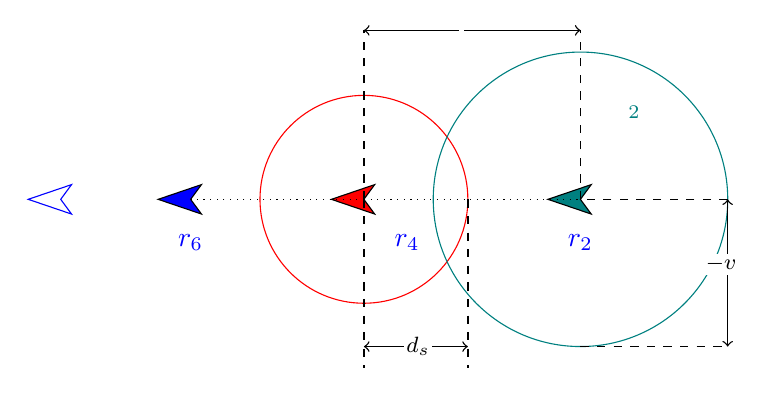
\begin{tikzpicture}[scale=1.1]
    \tikzstyle{ann} = [fill=white,font=\footnotesize,inner sep=1pt]
    % \useasboundingbox (1,0.5) rectangle (5.5,5);
    % center 2.875 2.75
    \coordinate (S) at (2.875, 2.75);
    \def\offset{0.5}
    \draw[fill=blue] (3,2.92) -- (2.5,2.75) -- (3,2.58) -- (2.875,2.75) -- cycle;
    \node[color=blue] at (2.875, 2.75-\offset) {$r_6$};
    % vacancy
    \def\dx{1.5}
    \def\ddx{2}
    \def\dddx{4.5}
    \coordinate (I) at (2.875+\ddx,2.75);
    \coordinate (C) at (2.875+\dddx,2.75);
    \draw[color=blue] (3-\dx,2.92) -- (2.5-\dx,2.75) -- (3-\dx,2.58) -- (2.875-\dx,2.75) -- cycle;
    \draw[fill=red] (3+\ddx,2.92) -- (2.5+\ddx,2.75) -- (3+\ddx,2.58) -- (2.875+\ddx,2.75) -- cycle;
    \node[color=blue] at (4.875+\offset, 2.75-\offset) {$r_4$};
    \draw[fill=teal] (3+\dddx,2.92) -- (2.5+\dddx,2.75) -- (3+\dddx,2.58) -- (2.875+\dddx,2.75) -- cycle;
    \node[color=blue] at (7.375, 2.75-\offset) {$r_2$};
    \draw[dotted] (I) -- (S);
    \draw[dotted] (I) -- (C);

    \def\safedist{1.2}
    \def\circleSafeI {(I) circle (\safedist)}
    \draw[color=red] \circleSafeI;
    \def\movedist{1.7}
    \def\circleMoveC {(C) circle (\movedist)}
    \draw[color=teal] \circleMoveC;
    % radius of circleMoveC
    \draw[dashed,line width=.5pt] (7.375, 2.75-\movedist) -- (7.375+\movedist,2.75-\movedist);
    \draw[dashed,line width=.5pt] (7.375+\movedist, 2.75) -- (7.375, 2.75);
    \draw[arrows=<->,line width=.5pt] (7.375+\movedist,2.75-\movedist) -- (7.375+\movedist,2.75);
    \node[ann] at (9,2) {$\range-v\dt$};
    \coordinate (Cu) at (7.375, 3+\movedist);
    \coordinate (Iu) at (4.875, 3+\movedist);
    \draw[dashed, line width=.5pt] (C) -- (Cu);
    \draw[dashed, line width=.5pt] (I) -- (Iu);
    \draw[arrows=<->, line width=.5pt] (Cu) -- (Iu);
    \node[ann] at (6, 3+\movedist) {$\range$};
    \coordinate (Id) at (4.875, 2.5-\movedist);
    \coordinate (M) at (4.875+\safedist, 2.75);
    \coordinate (Md) at (4.875+\safedist, 2.5-\movedist);
    \draw[dashed, line width=.5pt] (I) -- (Id);
    \draw[dashed, line width=.5pt] (M) -- (Md);
    \coordinate (Id2) at (4.875, 2.75-\movedist);
    \coordinate (Md2) at (4.875+\safedist, 2.75-\movedist);
    \draw[arrows=<->, line width=.5pt] (Id2) -- (Md2);
    \node[ann] at (5.5, 2.75-\movedist) {$d_s$};
    %%%%
    % \def\parentCircle {(S) circle (\movedist)}
    % \draw[color=blue] \parentCircle;
    % \node[color=blue] at (3,3.75) {$\B_s$};
    \node[color=teal] at (8,3.75) {$\B_2$}; 
        %%%%           
    %% \coordinate (X) at (3.5-\dx, 2.75);
    %% \coordinate (Xd) at (3.5-\dx,2.75-\movedist);
    %% \draw[arrows=<->, line width=.5pt] (X) -- (Xd);
    %% \node[ann] at (1.75,2) {$\range-v\dt$};
    %% \coordinate (Sd) at (2.875, 2.75-\movedist);
    %% \draw[dashed,line width=.5pt] (Xd) -- (Sd);
    %% \draw[dashed,line width=.5pt] (S) -- (X);
  \end{tikzpicture}
\end{minipage}
\begin{minipage}{0.9\linewidth}
  \centering
   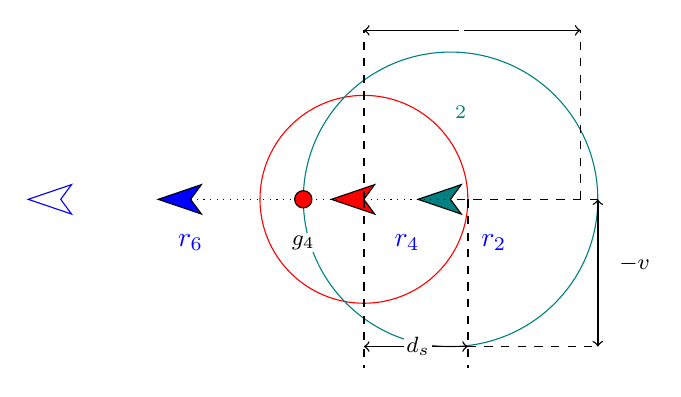
\begin{tikzpicture}[scale=1.1]
    \tikzstyle{ann} = [fill=white,font=\footnotesize,inner sep=1pt]
    % \useasboundingbox (1,0.5) rectangle (5.5,5);
    % center 2.875 2.75
    \coordinate (S) at (2.875, 2.75);
    \def\offset{0.5}
    \draw[fill=blue] (3,2.92) -- (2.5,2.75) -- (3,2.58) -- (2.875,2.75) -- cycle;
    \node[color=blue] at (2.875, 2.75-\offset) {$r_6$};
    % vacancy
    \def\dx{1.5}
    \def\ddx{2}
    \def\dddx{3}
    \coordinate (I) at (2.875+\ddx,2.75);  %4.375, 2.75
    \coordinate (C) at (2.875+\dddx,2.75); %5.875, 2.75
    \draw[color=blue] (3-\dx,2.92) -- (2.5-\dx,2.75) -- (3-\dx,2.58) -- (2.875-\dx,2.75) -- cycle;
    \draw[fill=red] (3+\ddx,2.92) -- (2.5+\ddx,2.75) -- (3+\ddx,2.58) -- (2.875+\ddx,2.75) -- cycle;
    \node[color=blue] at (4.875+\offset, 2.75-\offset) {$r_4$};
    \draw[fill=teal] (3+\dddx,2.92) -- (2.5+\dddx,2.75) -- (3+\dddx,2.58) -- (2.875+\dddx,2.75) -- cycle;
    \node[color=blue] at (5.875+\offset, 2.75-\offset) {$r_2$};
    \draw[dotted] (I) -- (S);
    \draw[dotted] (I) -- (C);

    \def\safedist{1.2}
    \def\circleSafeI {(I) circle (\safedist)}
    \draw[color=red] \circleSafeI;
    \def\movedist{1.7}
    \def\circleMoveC {(C) circle (\movedist)}
    \draw[color=teal] \circleMoveC;
    %%%%%%%%%%%%%%%%
    \coordinate (Cu) at (7.375, 3+\movedist);
    \coordinate (Iu) at (4.875, 3+\movedist);
    \coordinate (Co) at (7.375, 2.75);
    \draw[dashed, line width=.5pt] (Co) -- (Cu);
    \draw[dashed, line width=.5pt] (I) -- (Iu);
    \draw[arrows=<->, line width=.5pt] (Cu) -- (Iu);
    \node[ann] at (6, 3+\movedist) {$\range$};
    \coordinate (Id) at (4.875, 2.5-\movedist);
    \coordinate (M) at (4.875+\safedist, 2.75);
    \coordinate (Md) at (4.875+\safedist, 2.5-\movedist);
    \draw[dashed, line width=.5pt] (I) -- (Id);
    \draw[dashed, line width=.5pt] (M) -- (Md);
    \coordinate (Id2) at (4.875, 2.75-\movedist);
    \coordinate (Md2) at (4.875+\safedist, 2.75-\movedist);
    \draw[arrows=<->, line width=.5pt] (Id2) -- (Md2);
    \node[ann] at (5.5, 2.75-\movedist) {$d_s$};
    %%%%%%%%%%%%%%%%%
    \coordinate (N) at (5.875+\movedist, 2.75);
    \coordinate (Nd) at (5.875+\movedist, 2.75-\movedist);
    \draw[dashed,line width=.5pt] (N) -- (C);
    \draw[dashed,line width=.5pt] (Md2) -- (Nd);
    % radius of circleMoveC
    \draw[arrows=<->,line width=.5pt] (N) -- (Nd);
    \node[ann] at (8,2) {$\range-v\dt$};
    %%%% G.x = c.x - \movedist
    \coordinate (G) at (5.875-\movedist, 2.75);
    \draw[fill=red] (G) circle (0.1);
    \node[ann] at (5.875-\movedist, 2.75-\offset) {$g_4$};
    %%%%
    % \def\parentCircle {(S) circle (\movedist)}
    % \draw[color=blue] \parentCircle;
    %%%%
    %\node[color=blue] at (3,3.75) {$\B_s$};
    \node[color=teal] at (6,3.75) {$\B_2$}; 
    %% \coordinate (X) at (3.5-\dx, 2.75);
    %% \coordinate (Xd) at (3.5-\dx,2.75-\movedist);
    %% \draw[arrows=<->, line width=.5pt] (X) -- (Xd);
    %% \node[ann] at (1.75,2) {$\range-v\dt$};
    %% \coordinate (Sd) at (2.875, 2.75-\movedist);
    %% \draw[dashed,line width=.5pt] (Xd) -- (Sd);
    %% \draw[dashed,line width=.5pt] (S) -- (X);
    \end{tikzpicture}
\end{minipage}
   \caption{(top) The relocate robot $r_4$ intends to move to the
   vacancy (hollow arrow) of the root robot $r_6$. Robot $r_2$ is a
   child of $r_4$. Since $\operatorname{dist}(r_4, r_2) > d_s$, $r_4$
   waits for $r_2$ to move close to it. (bottom) When
   $\operatorname{dist}(r_4, r_2) \leq d_s$, the relocate robot $r_4$
   finds the closest point $g_4 \in \B_2$ (red dot)
   to the vacancy as an intermediate goal.}